% \chapter{Axionlike-particle-induced spin precession}\label{chap:theory}

\section{Earth-bound ALPs}\label{sec:theory:earthALP}

% % \subsection{Gravitational atom}

% mention total mass constrained by the astro observation. 

% \YZ{include lambdadB of axion trapped in gravitational potential (mention earth potential first with plots) of items such as Sun or Earth. what can be the mechanism of trapping and accumulation of DM? }

% in the case of earth, the wavelength is very large. It can be treated like an atom. 

% Schroedinger eq for deriving the probability / mass distribution. 

% numeric solution of schr. eq.

% get gradient from the wavefunction -> corresponding Omega_a's. plus linewidth

% with plots. 

% ground state, excitated states.... coherence time if multiple modes are interfering. 


% % \subsection{Coherence time}  % for MW axion

% \subsection{Daily modulations} % due to the earth rotation

The galactic dark-matter halo provides the primary ALP signal target discussed in Chapter~\ref{chap:results}.
However, a distinct and potentially enhanced source arises from ALPs that are gravitationally bound to the Earth.
Such Earth-bound states are analogous to atomic bound states---the Earth's gravitational potential plays the role of the Coulomb well and the ALP plays the role of the electron---and can support a discrete spectrum of spatial eigenstates.
This section derives the properties of these bound states, estimates the resulting spin-precession signal, and discusses the characteristic daily modulation that distinguishes this signal from the galactic background.

\subsection{Trapping and accumulation of dark matter}\label{sec:theory:earthALP:trapping}

For Earth-bound states to be populated, ALPs from the galactic halo must lose enough kinetic energy to fall below the local escape velocity ($v_\mathrm{esc} \approx \SI{11.2}{\km\per\s}$ for Earth).
Several mechanisms have been proposed \YZ{cite: Banerjee et al.\ 2019 arXiv:1902.07720; OHare 2025 fine-grained; other relevant papers}:

\begin{description}
    \item[Gravitational three-body scattering] A galactic ALP passing near the Earth can scatter off a third body (e.g.\ the Sun or Moon), losing kinetic energy and becoming trapped in a bound orbit.
    The rate depends on the local density and the ALP-body cross section.
    \item[Self-interaction or wave-packet spreading] \YZ{placeholder: if ALPs have self-interactions or if wave-packet decoherence provides an effective dissipation, this may also populate bound states.}
    \item[Resonant capture] Near specific orbital resonances the exchange of energy between the ALP and the Earth-Moon or Earth-Sun system may be efficient.
\end{description}

The total mass $M_\mathrm{bound}$ of ALPs trapped in Earth-bound states is strongly constrained by astrophysical and geophysical observations \YZ{leave the plot here.
cite and expand: relevant constraints on exotic mass inside Earth from geophysics / seismology / gravitational measurements}.
An upper bound comes from the requirement that the Earth's measured gravitational multipole moments not be distorted beyond current geodetic precision.
\YZ{Add quantitative upper limit on $M_\mathrm{bound}$ once reference is identified.}
\YZ{We note that.... skip the mechanism of capturing...}
\begin{figure}
    \centering
    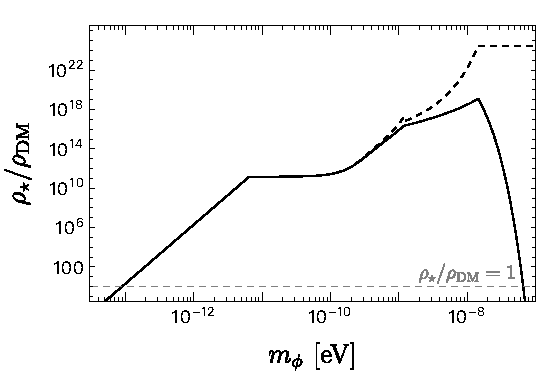
\includegraphics[scale =0.9]{figures/MaxDensity_EH.pdf}
    \caption{Density Distribution of ground state Earth-bound ALP halo.
    The solid line indicates the density at the Earth surface, whereas the dashed line represents the density at the center of the halo.
    The density value $\rho_\star$ is derived from the maximum Earth ALP halo mass permitted by gravitational constraints, as assessed in \cite{banerjee_relaxion_2020,banerjee_searching_2020}.}%
    \label{fig:groundstate_density}%
\end{figure}
\YZ{check if max dm mass is mentioned}
\subsection{Gravitational potential and the quantum picture}  %  and the Bohr radius

To simplify the calculation, Earth is considered as a spherical object.
The density of Earth varys over radii.
From geophysical measurements on earthquake waves, Preliminary reference Earth model (PREM)\cite{Dziewonski1981_PREM} was constructed, giving the Earth density profile as shown in Figure~\ref{fig:PREM}.
\begin{figure}
    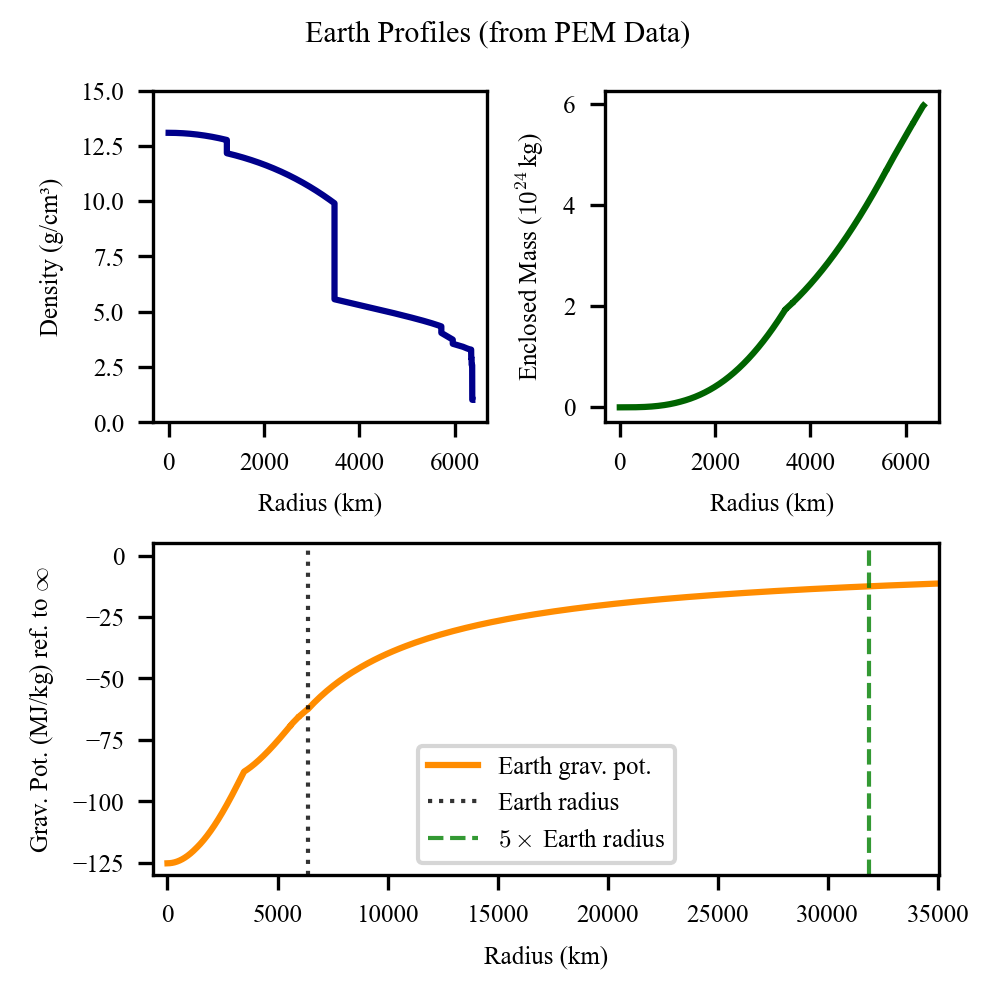
\includegraphics[width=\linewidth]{figures/Earth_Profiles_(PEM_Data).png}
    \caption{to be modified later.}
    \label{fig:PREM}
\end{figure}

The gravitational potential of Earth $V_g / m$ per unit mass can be found by
\begin{equation}
    V_g(r) / m = -\frac{G M_\mathrm{enclosed}}{r}~,
    \label{eq:grav_potential}
\end{equation}
\YZ{check if we are wrong by a constant or so. }
where $r$ is the distance measured from the Earth's center, $G$ is Newton's constant, and $M_\mathrm{enclosed}$ is the Earth's mass enclosed by $r$.
Here we take the infinity as the reference point and have potential $V_g(\infty)/m=\SI{0}{\joule\per\kg}$.
The potential over radii can be calculated numerically based on PREM (Figure~\ref{fig:PREM}).
The Earth escape velocity can therefore be found by
\begin{equation}
    v_\mathrm{escape} = \sqrt{\frac{2 G M_\oplus}{R_\oplus}~}, 
    \label{eq:earth_escape_velocity}
\end{equation}
where $M_\oplus=\SI{6e24}{\kg}$ and $R_\oplus=\SI{6378.1}{\km}$ are the mass and average radius of Earth, respectively.
By plugging the values, the Earth escape velocity is found to be \SI{11.2}{\km/\second}.
Since the escape speed is much smaller than the speed of light, non-relativistic limit is assumed for the discussion.

% \subsection{The quantum picture}  %  of Earth-bound ALP
% why do we have to look at ALP bound by Earth in the quantum picture
For ultralight dark matter particles bound by Earth, they can no longer be treated as classic objects due to their large de~Broglie wavelengths.
A rough estimation of the wavelength is made as follows.
% The speed of ALP should not exceed
The ALP masses that CASPEr-G can probe range from $\sim\SI{4}{\pico\eV}$ to $\SI{2.5}{\micro\eV}$.
Consider ALPs trapped by the earth potential with velocities roughly smaller than the escape veclocity.
% Consider ultralight particles with mass $<\SI{10}{\eV/c^2}$ trapped by the earth potential. 
% Their kinetic energy must be comparable or even smaller than the potential energy, as
% \begin{equation}
%     E_k = \frac{1}{2} m_a v_a^2 \lesssim \frac{G M_\mathrm{enclosed} m_a}{r}~.
% \end{equation}
% The maximum of the absolute potential energy ${G M_\mathrm{enclosed} m_a}/{r}$\YZ{change enclosed mass to M(r)?} is ${G M_\oplus \SI{10}{\eV/c^2}}/{R_\oplus} = \SI{7e-9}{\eV}$. This transfers to $v_a\lesssim v_\mathrm{esc} = \SI{11.2}{\km/\second}$. 
The de~Broglie wavelength as a function of particle mass $\lambda_\mathrm{dB}(m_a, v_a) = \frac{h}{m_a v_a}$ gives
\begin{itemize}
    \item $\lambda_\mathrm{dB}(\SI{4}{\pico\eV}, \SI{11.2}{\km/\second}) \approx \SI{8.3e9}{\m} \approx 1300 R_\oplus$ and
    \item $\lambda_\mathrm{dB}(\SI{2.5}{\micro\eV}, \SI{11.2}{\km/\second}) \approx \SI{13}{\km} \approx 0.0021 R_\oplus$.
\end{itemize}
Therefore, across the scan range of CASPEr, the de~Broglie wavelength spans values from much smaller to much larger than the Earth radius.
In later chapters, a measurement probing MHz ALPs is presented.
This corresponds to a de~Broglie wavelength $\sim\SI{1}{R_\oplus}$.
To prepare for the analysis, we focus on this scenario and take the wave nature into account.
\YZ{mention Na here. }

\subsection{Bound-state wavefunctions}\label{sec:theory:earthALP:wavefunctions}

The general relation between an ALP wavefunction, its local energy density, and the real scalar field was established in Equations~\eqref{eq:a0_Psi_real} and~\eqref{eq:a0_rhoDM_Psi_real}.
For the Earth-bound model, the wavefunction is expanded in the discrete gravitational eigenstates:
\begin{equation}
    \Psi(\mathbf{r}, t) = e^{-i m_a c^2 t / \hbar}\sum_{nlm}^{} c_{nlm} e^{-i E_n t / \hbar} \psi_{nlm}(\mathbf{r})\,.
    \label{eq:Psi_r_t}
\end{equation}
Here $\Psi(\mathbf{r}, t)$ is the wavefunction, $\psi_{nlm}$ and $E_n$ are the eigenfunction and energy of the state $(n,\,l,\,m)$, and $c_{nlm}$ are expansion coefficients determined by the state populations.
The total particle number $N_a$ enters through the density below.
The fast oscillation at ALP Compton frequency is indicated by $e^{-i m_a c^2 t / \hbar}$, where the small variation of oscillation frequency is indicated by $e^{-i E_n t / \hbar}$.
The corresponding local density, $\rho_{DM}^{E}(\mathbf{r})=m_a c^2N_a
\langle|\Psi(\mathbf{r},t)|^2\rangle_t$, fixes the field amplitude through
Equation~\eqref{eq:a0_rhoDM_Psi_real}.
The remaining task is therefore to determine the eigenfunctions, eigenenergies, and state populations in the Earth's potential.

In the non-relativistic limit, the eigenstates can be found by the time-independent Schrödinger equation (TISE)
\begin{equation}
    \left[-\frac{\hbar^2}{2 m_a}\nabla^2 + V_g(r)\right]\psi_{nlm}(\mathbf{r})
    = E_n\,\psi_{nlm}(\mathbf{r})
    \,.\label{eq:schrodinger_earth}
\end{equation}
In analogy to the hydrogen atom, the ALP-Earth system is a gravitational atom \YZ{cite: relevant paper on gravitational atom, e.g.\ Arvanitaki et al. and more...}.
\YZ{what about quantum number m? zero?}

%%%% %%%% %%%% %%%% %%%% %%%% %%%% %%%% %%%% %%%%   %%%% %%%% %%%% %%%% %%%% %%%% %%%% %%%% %%%% %%%% 
%%%% %%%% the following text is about the Bohr radius. We may or may not need to include it %%%% %%%% 
% , with the fine-structure constant replaced by the gravitational coupling
% \begin{equation}
%     \alpha_g \equiv \frac{GM_E\,m_a}{\hbar c}
%     \approx 2\times10^{-5}\left(\frac{m_a}{\SI{1}{\micro\eV}}\right)
%     \,.\label{eq:alpha_g}
% \end{equation}
% The analogue of the Bohr radius is
% \begin{equation}
%     a_g = \frac{\hbar^2}{GM_E\,m_a^2}
%     = \frac{\hbar c}{m_a c^2\,\alpha_g}
%     \approx \SI{283}{\km}\left(\frac{\SI{5.58}{\nano\eV}}{m_a}\right)^2
%     \,,\label{eq:bohr_radius_grav}
% \end{equation}
% and the bound-state energy levels are
% \begin{equation}
%     E_n = -\frac{m_a c^2\,\alpha_g^2}{2n^2}
%     = -\frac{G^2M_E^2\,m_a^3}{2\hbar^2\,n^2}
%     \,,\quad n = 1,2,3,\ldots
%     \label{eq:energy_levels_earth}
% \end{equation}

% The Bohr radius $a_g$ sets the spatial extent of the ground state. Its scaling as $m_a^{-2}$ means it varies rapidly with mass:
% \begin{itemize}
%     \item For $m_a \lesssim \SI{1}{\nano\eV}$: $a_g \gtrsim R_E$ --- the ground-state wavefunction extends to or beyond the Earth's surface; the ALP is loosely bound and the signal at the surface is sensitive to the full volume integral.
%     \item For $m_a \sim \SI{5}{\nano\eV}$: $a_g \sim \SI{300}{\km} \ll R_E$ --- the ALP is tightly bound inside the Earth; the surface gradient is set by the exponential tail of the wavefunction.
%     \item For $m_a \gg \SI{10}{\nano\eV}$: $a_g \ll R_E$ --- increasingly localized deep inside the Earth; detectors at the surface probe only the far tail.
% \end{itemize}
% \YZ{Add figure: Earth gravitational potential well as a function of radius $r$, overlaid with the ground-state probability density $|\psi_{100}|^2$ for one or two representative masses. Script: \texttt{scripts-and-data/earth\_ALP\_wavefunction.py} (to be written).}
%%%% %%%% %%%% %%%% %%%% %%%% %%%% %%%% %%%% %%%% %%%% %%%% %%%% %%%% %%%% %%%% %%%% %%%% %%%% %%%% %%%% 

Considering the spherical symmetry of the Earth gravitational potential, spherical coordinate system $(r, \theta, \varphi)$ is adopted, where $r$ is the radial distance from the origin, $\theta$ is the polar angle, and $\varphi$ is the azimuthal angle.
In spherical coordinates,
\begin{equation}
    \nabla^2 = \frac{1}{{r}^2}\frac{\partial}{\partial r}\left(r^2\frac{\partial}{\partial r}\right)+\frac{1}{r^2\sin\theta}\frac{\partial}{\partial \theta}\left(\sin\theta\frac{\partial}{\partial \theta}\right)+\frac{1}{r^2\sin^2\theta}\frac{\partial^2}{\partial \varphi^2}
    \,,\label{eq:laplacian_spherical}
\end{equation}
so that TISE can be rewritten as
\begin{equation}
    \left[-\frac{\hbar^2}{2m}\left(\frac{1}{{r}^2}\frac{\partial}{\partial r}\left(r^2\frac{\partial}{\partial r}\right)-\frac{{\hat{L}}^2}{\hbar^2r^2}\right)+V_g(r)\right]\psi_{nlm}\left(r,\ \theta,\varphi\right)=E_{n}\psi_{nlm}\left(r,\ \theta,\varphi\right)\,,
\end{equation}
where $\hat{L}$ is the angular momentum operator.
The eigen-function can be separated as
\begin{equation}
    \psi_{nlm}(\mathbf{r}) = R_{nl}(r)\,Y_l^m(\hat{\mathbf{r}})
    \,,\label{eq:psi_R_Y}
\end{equation}
where $R_{nl}$ is the radial wavefunction and $Y_l^m$ is the spherical harmonic.
The spherical harmonics satisfies
\begin{equation}
    {\hat{L}}^2Y\left(\theta,\ \varphi\right)=l\left(l+1\right)\hbar^2Y\left(\theta,\varphi\right)\,.
\end{equation}
Therefore, to derive the radial wavefunction of eigen-state with angular quantum number $l$, TISE is transformed to
\begin{equation}
    -\frac{\hbar^2}{2m}\frac{1}{{r}^2}\frac{\partial}{\partial r}\left[r^2\frac{\partial R_{nl}\left(r\right)}{\partial r}\right]+\left[\frac{l\left(l+1\right)\hbar^2}{2mr^2}+V_g\right]R_{nl}\left(r\right)=E_{n}R_{nl}\left(r\right)\,.
    \label{eq:TISE_R}
\end{equation}
Since the earth density is not uniform, it is difficult to derive the radial wavefunction analytically.
Hence, numerical method is adopted.
In a discretized space, a matrix for the Hamiltonian in Equation\,\eqref{eq:TISE_R} is constructed.
The eigen-values (eigen-energies) and eigen-vectors (eigen-states) can be derived using Python package \texttt{SciPy}.
This method is implemented in the Python class \texttt{EarthBoundAxionHalo} of \texttt{axionbloch}.

Note that normalization is necessary for deriving the right magnitude of the eigen-functions.
The wavefunctions are normalized so that the total probability integrates to unity,
\begin{equation}
    \int|\psi_{nlm}(\mathbf{r})|^2\,d^3r
    = \int_0^\infty |R_{nl}(r)|^2\,r^2\,dr
    \int|Y_l^m(\hat{\mathbf{r}})|^2\,d\Omega
    = 1
    \,.\label{eq:psi_norm}
\end{equation}
% \begin{align}
%     \int_0^\infty |R_{nl}|^2 r^2\,dr = 1
%     \,.\label{eq:psi_norm}
% \end{align}
% \begin{align}
%     \int|Y_l^m|^2\,d\Omega = 1
%     \,.\label{eq:psi_norm}
% \end{align}
Here $\Omega$ is solid angle coordinate.
% The two factors are independently normalized: $\int_0^\infty |R_{nl}|^2 r^2\,dr = 1$ and $\int|Y_l^m|^2\,d\Omega = 1$.
Examples of normalized wavefunctions are illustrated in Figure~\ref{fig:wavefunctions}.
\begin{figure}
    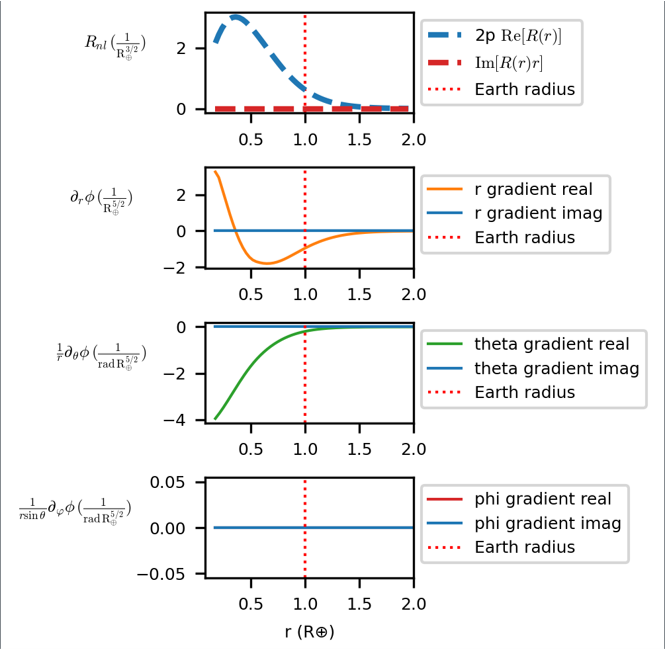
\includegraphics[width=0.45\textwidth]{figures/wavefunction-2p.png}
    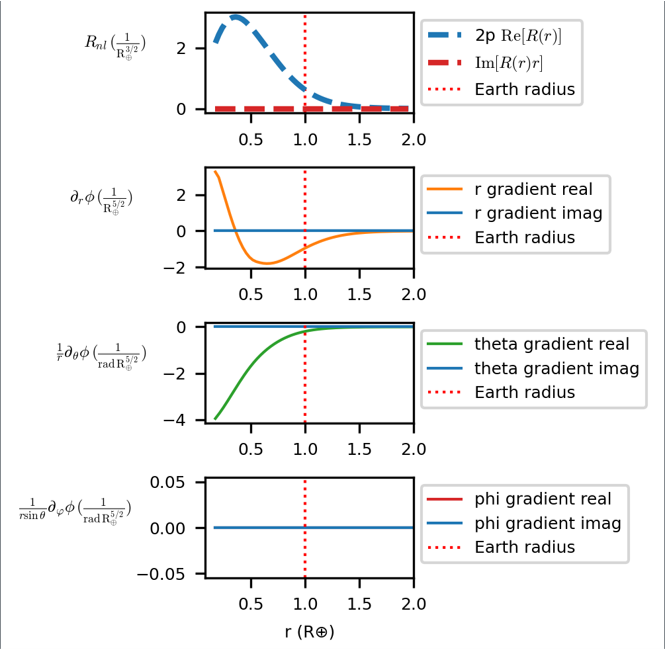
\includegraphics[width=0.45\textwidth]{figures/wavefunction-2p.png}
    \caption{radial wavefunctions of 1s 2p... states.
    include higher states and mention that we are only interested in low energy states.}
    \label{fig:wavefunctions}
\end{figure}
\YZ{eigen states plotted here:} % C:\Users\zhenf\D\Yu0702\AxionBloch\examples\example_EarthBoundAxionHalo-plot-rR_nl.py

% in terms of associated Laguerre polynomials with $r$ scaled by $a_g$. The ground state ($n=1$, $l=m=0$) is
% \begin{equation}
%     \psi_{100}(\mathbf{r}) = \frac{1}{\sqrt{\pi}\,a_g^{3/2}}\,e^{-r/a_g}
%     \,.\label{eq:psi_ground}
% \end{equation}
% The local ALP field amplitude at the detector is proportional to $|\psi_{nlm}|$ evaluated at the detector position $\mathbf{r}_\mathrm{det}$ (for a mode carrying total energy $E_n$ and a fixed number of bound quanta).

% The gradient of the ALP field, which drives nuclear spin precession through Equation~\eqref{eq:HaNN}, is
% \begin{equation}
%     \boldsymbol{\nabla}a\big
%     \propto \boldsymbol{\nabla}\psi_{nlm}\big
%     \,.\label{eq:earth_ALP_gradient}
% \end{equation}
% For the ground state, $|\boldsymbol{\nabla}\psi_{100}| = |\psi_{100}|/a_g$, so the gradient and the amplitude are related by a factor $1/a_g$.

% The corresponding r.m.s.\ Rabi frequency \YZ{derive more carefully; the expression below assumes the total bound mass $M_\mathrm{bound}$ is known}
% \begin{equation}
%     \Omega_a^\mathrm{Earth} \approx g_\mathrm{aNN}\,\frac{|\boldsymbol{\nabla}\psi_{100}(\mathbf{r}_\mathrm{det})|}{\gamma}\,
%     \sqrt{\frac{2M_\mathrm{bound}\,c^2}{m_a}}
%     \,.\label{eq:Omega_earth}
% \end{equation}

\subsection{ALP field gradient}\label{sec:theory:earthALP:gradient}

The ALP field gradient at the detector can be derived from the spatial gradient of the wavefunction $\psi_{nlm}$ evaluated at the detector position.
The gradient operator in spherical coordinates is
\begin{equation}
    \boldsymbol{\nabla} = \hat{\mathbf{r}}\,\frac{\partial}{\partial r} + \hat{\boldsymbol{\theta}}\,\frac{1}{r}\frac{\partial}{\partial \theta} + \hat{\boldsymbol{\varphi}}\,\frac{1}{r\sin\theta}\frac{\partial}{\partial \varphi}
    \,.\label{eq:gradient_spherical}
\end{equation}
The eigenstates are defined in the Earth-rest frame, whereas the gradient coupling is measured in the laboratory frame $L$.
Since the ALP field is a Lorentz scalar, $a'(x')=a(x)$, while its derivatives transform according to the inverse Lorentz transformation.
Applying the chain rule, $\partial'_\mu=(\Lambda^{-1})^\nu{}_\mu\partial_\nu$, mixes the temporal derivative with the component of the spatial gradient parallel to the laboratory velocity.
Here $\Lambda^\mu{}_\nu$ is the $4\times4$ Lorentz-boost matrix relating the Earth-rest-frame coordinates $x^\mu=(ct,\mathbf{r})$ to the laboratory-frame coordinates through $x'^\mu=\Lambda^\mu{}_\nu x^\nu$.
Its inverse appears because the derivative basis transforms oppositely to the coordinates; the Greek indices run over the temporal and three spatial components.
To obtain the spatial transformation explicitly, the unboosted gradient is decomposed into components parallel and perpendicular to $\mathbf{v}$:
\begin{equation}
    \boldsymbol{\nabla}_{\parallel}a
    =
    \frac{\mathbf{v}}{v^2}
    \left(\mathbf{v}\cdot\boldsymbol{\nabla}a\right),
    \qquad
    \boldsymbol{\nabla}_{\perp}a
    =
    \boldsymbol{\nabla}a-\boldsymbol{\nabla}_{\parallel}a
    \,.
\end{equation}
The inverse Lorentz boost leaves the perpendicular component unchanged and transforms the parallel component as
\begin{equation}
    \left(\boldsymbol{\nabla}_{L}a\right)_{\perp}
    =
    \boldsymbol{\nabla}_{\perp}a,
    \qquad
    \left(\boldsymbol{\nabla}_{L}a\right)_{\parallel}
    =
    \gamma_L
    \left(
    \boldsymbol{\nabla}_{\parallel}a
    +
    \frac{\mathbf{v}}{c^2}\partial_t a
    \right)
    \,.
\end{equation}
Adding these two components gives
\begin{equation}
    \boldsymbol{\nabla}_{L}a
    =
    \boldsymbol{\nabla}a
    +\frac{\gamma_L-1}{v^2}\mathbf{v}
    \left(\mathbf{v}\cdot\boldsymbol{\nabla}a\right)
    +\gamma_L\frac{\mathbf{v}}{c^2}\partial_t a
    \,,\label{eq:gradient_lorentz_boost}
\end{equation}
where $\mathbf{v}$ is the velocity of the laboratory relative to the Earth-rest frame and $\gamma_L=(1-v^2/c^2)^{-1/2}$.
In the limit $v/c\to0$, the laboratory and Earth-rest frames coincide.
Although the second term in Equation~\eqref{eq:gradient_lorentz_boost} contains $v^2$ in the denominator, $\gamma_L-1\propto v^2/c^2$, and the complete term has the regular limit
\begin{equation}
    \lim_{v\to0}
    \frac{\gamma_L-1}{v^2}\mathbf{v}
    \left(\mathbf{v}\cdot\boldsymbol{\nabla}a\right)
    =0
    \,.
\end{equation}
The temporal-gradient term also vanishes, so Equation~\eqref{eq:gradient_lorentz_boost} reduces to
\begin{equation}
    \boldsymbol{\nabla}_{L}a=\boldsymbol{\nabla}a
    \qquad (v=0)
    \,,
\end{equation}
as expected.

For $0<v/c\ll1$, the Lorentz factor can be expanded as
\begin{equation}
    \gamma_L
    =1+\frac{1}{2}\frac{v^2}{c^2}
    +\mathcal{O}\left(\frac{v^4}{c^4}\right),
    \qquad
    \frac{\gamma_L-1}{v^2}
    =\frac{1}{2c^2}
    +\mathcal{O}\left(\frac{v^2}{c^4}\right)
    \,.
\end{equation}
Consequently,
\begin{equation}
    \boldsymbol{\nabla}_{L}a
    =
    \boldsymbol{\nabla}a
    +\frac{\mathbf{v}}{c^2}\partial_t a
    +\frac{\mathbf{v}}{2c^2}
    \left(\mathbf{v}\cdot\boldsymbol{\nabla}a\right)
    +\cdots
    \,.
\end{equation}
To first order in $v/c$, this becomes
\begin{equation}
    \boldsymbol{\nabla}_{L}a
    \simeq
    \boldsymbol{\nabla}a
    +\frac{\mathbf{v}}{c^2}\partial_t a
    \,.
\end{equation}
The condition $v/c\ll1$ does not necessarily make the temporal-gradient contribution negligible because $\partial_t a$ contains the rapid ALP Compton oscillation.
It is the laboratory-frame gradient $\boldsymbol{\nabla}_{L}a$ that enters the interaction Hamiltonian in Equation~\eqref{eq:HaNN}.
The unboosted gradient can be inferred from Equations~\eqref{eq:a0_Psi_real} and~\eqref{eq:Psi_r_t} as
\begin{align}
    \boldsymbol{\nabla}a(\mathbf{r}, t)
    &= \sqrt{\frac{N_a \hbar^3 c}{2 m_a}} \Re\left[ \boldsymbol{\nabla} \Psi(\mathbf{r}, t) \right] \\
    &= \sqrt{\frac{N_a \hbar^3 c}{2 m_a}} \Re\left[ e^{-i m_a c^2 t / \hbar}\sum_{nlm}^{} c_{nlm} e^{-i E_n t / \hbar} \boldsymbol{\nabla}\psi_{nlm}(\mathbf{r}) \right]
    \,,\label{eq:gradient_Psi_sum}
\end{align}
where
% \begin{equation}
%     a_0(\mathbf{r}, t) = \sqrt{\frac{N_a \hbar^3 c}{2 m_a}} \left(\Psi(\mathbf{r}, t) + \Psi^*(\mathbf{r}, t) \right)~, 
%     \label{eq:a0_Psi_real_imag}
% \end{equation}
% where
% \begin{equation}
%     \Psi(\mathbf{r}, t) = e^{-i m_a c^2 t / \hbar}\sum_{nlm}^{} c_{nlm} e^{-i E_n t / \hbar} \psi_{nlm}(\mathbf{r})\,.
%     \label{eq:Psi_r_t}
% \end{equation}
\begin{equation}
    \boldsymbol{\nabla}\psi_{nlm}(\mathbf{r})       
    = \hat{\mathbf{r}}\,\frac{\partial R_{nl}}{\partial r}Y_l^m + \hat{\boldsymbol{\theta}}\,\frac{R_{nl}}{r}\frac{\partial Y_l^m}{\partial \theta} + \hat{\boldsymbol{\varphi}}\,\frac{R_{nl}}{r\sin\theta}\frac{\partial Y_l^m}{\partial \varphi}
    \,.\label{eq:gradient_psi_nlm}
\end{equation}
Using Equation~\eqref{eq:Psi_r_t}, the two Lorentz-boost terms in Equation~\eqref{eq:gradient_lorentz_boost} become
\begin{align}
    \frac{\gamma_L-1}{v^2}\mathbf{v}
    \left(\mathbf{v}\cdot\boldsymbol{\nabla}a\right)
    &=
    \sqrt{\frac{N_a \hbar^3 c}{2 m_a}}
    \Re\left[
    e^{-i m_a c^2 t/\hbar}
    \sum_{nlm} c_{nlm}e^{-iE_nt/\hbar}
    \frac{\gamma_L-1}{v^2}\mathbf{v}
    \left(\mathbf{v}\cdot\boldsymbol{\nabla}\psi_{nlm}\right)
    \right],
    \\
    \gamma_L\frac{\mathbf{v}}{c^2}\partial_t a
    &=
    \sqrt{\frac{N_a \hbar^3 c}{2 m_a}}
    \Re\left[
    e^{-i m_a c^2 t/\hbar}
    \sum_{nlm} c_{nlm}e^{-iE_nt/\hbar}
    \left(
    -i\gamma_L\frac{m_a c^2+E_n}{\hbar c^2}
    \mathbf{v}\,\psi_{nlm}
    \right)
    \right]
    \,.\label{eq:gradient_boost_terms_Psi}
\end{align}
The size of these corrections can be estimated from the rotation of the Earth.
Using $R_\oplus\simeq\SI{6.37e6}{\meter}$ and the sidereal rotation period $T_\oplus\simeq\SI{8.62e4}{\second}$ gives the maximum surface speed
\begin{equation}
    v_\mathrm{rot}^{\max}
    =
    \frac{2\pi R_\oplus}{T_\oplus}
    \simeq\SI{4.65e2}{\meter\per\second},
    \qquad
    \frac{v_\mathrm{rot}^{\max}}{c}
    \simeq 1.55\times10^{-6}
    \,.
\end{equation}
At latitude $\lambda$, this speed is reduced by a factor $\cos\lambda$.
The corresponding Lorentz factor satisfies
\begin{equation}
    \gamma_L-1
    \simeq
    \frac{1}{2}\left(\frac{v_\mathrm{rot}^{\max}}{c}\right)^2
    \simeq 1.2\times10^{-12}
    \,,
\end{equation}
so the first correction in Equation~\eqref{eq:gradient_boost_terms_Psi} is negligible compared with the unboosted gradient.
For an ALP field oscillating at ordinary frequency $\nu_a$, the time-derivative term instead produces an effective gradient
\begin{equation}
    \frac{\left|\delta\boldsymbol{\nabla}a\right|_t}{|a|}
    \sim
    \frac{2\pi\nu_a v_\mathrm{rot}^{\max}}{c^2}
    \simeq
    \frac{0.21}{R_\oplus}
    \left(\frac{\nu_a}{\SI{1}{\mega\hertz}}\right)
    \,.
\end{equation}
Relative to an intrinsic bound-state gradient characterized by a speed
$v_\mathrm{bound}$, the temporal boost contribution is approximately
$v_\mathrm{rot}/v_\mathrm{bound}$.
For $v_\mathrm{bound}\sim v_\mathrm{esc}=\SI{11.2}{\kilo\meter\per\second}$,
this ratio is about $4\%$ at the equator.
The correction proportional to $\gamma_L-1$ is therefore of order
$10^{-12}$, whereas the temporal boost correction is of order $4\%$ for
this velocity scale and can be larger when the intrinsic transverse
gradient is suppressed.

The laboratory velocity relative to the Earth-bound halo is written generally as
\begin{equation}
    \mathbf{v}
    =
    v_r\hat{\mathbf{r}}
    +v_\theta\hat{\boldsymbol{\theta}}
    +v_\varphi\hat{\boldsymbol{\varphi}},
    \qquad
    v^2=v_r^2+v_\theta^2+v_\varphi^2
    \,,
\end{equation}
where the radial, polar, and azimuthal components are all retained.
The boost correction to the complex gradient amplitude of one mode is then
\begin{equation}
    \begin{aligned}
        \delta\boldsymbol{\mathcal{G}}_{nlm}
        &=
        \frac{\gamma_L-1}{v^2}\mathbf{v}
        \left(
        v_r\frac{\partial R_{nl}}{\partial r}Y_l^m
        +v_\theta\frac{R_{nl}}{r}\frac{\partial Y_l^m}{\partial\theta}
        +v_\varphi\frac{R_{nl}}{r\sin\theta}\frac{\partial Y_l^m}{\partial\varphi}
        \right)
        \\
        &\quad
        -i\gamma_L\frac{\omega_n}{c^2}
        \mathbf{v}R_{nl}Y_l^m
        \,,
        \qquad
        \omega_n=\frac{m_a c^2+E_n}{\hbar}
        \,.
    \end{aligned}
    \label{eq:gradient_boost_mode}
\end{equation}
For the spherically symmetric state with $l=m=0$, the angular derivatives vanish, but the first correction retains a radial contribution proportional to $v_r\,\partial R_{n0}/\partial r$.
It vanishes only when $v_r=0$, while the contribution from the temporal derivative remains.
If multiple modes are populated, the total gradient is a superposition of the gradients from each mode, weights of which correspond to the population distribution, as can be seen in Equation~\eqref{eq:gradient_Psi_sum}.
%  and Equation~\ref{eq:psi_R_Y} 

contributed by the wavefunction $\psi_{nlm}$

The gradient magnitude depends on the eigen-state $(n, l, m)$ and the detector location.
The characteristics of the gradient are addressed as follows:
\begin{itemize}
    \item For the eigen-states with zero angular momentum ($s$ state), the wavefunction is spherically symmetric, so the gradient is purely radial and its magnitude is proportional to the radial wavefunction gradient\YZ{is this paragraph right??}.
    \item When angular momentum is non-zero ($l>=1$), the gradient has non-radial components may vary over different locations, depending on the angular structure of the wavefunction.
    \item The choice of the quantization axis is critical for considering $l>0$ states.
    Since the solar gravity breaks the rotational symmetry, the $z$-axis is chosen along the Earth--Sun line.
    The $x$-axis is chosen along the instantaneous velocity of the Earth in the Solar System, and the $y$-axis is defined by $\hat{\mathbf{y}}=\hat{\mathbf{z}}\times\hat{\mathbf{x}}$.
    This coordinate system generally does not align with the Earth's rotation axis, so the laboratory velocity is retained in all three spherical components, $v_r$, $v_\theta$, and $v_\varphi$.
    The gradient at the detector location therefore exhibits a daily modulation as the Earth rotates, as discussed in Section~\ref{sec:theory:earthALP:periodic}.
    \item \textbf{Azimuthal dependence} For modes with $m\neq 0$, the gradient has an azimuthal dependence.
    However, for the brevity of this discussion, only $m=0$ is considered in this work.
\end{itemize}
The values of the gradients are computed numerically from the eigen-states and are used to estimate the expected signal strength in Chapter~\ref{chap:results}.
\YZ{mention the time for computing the gradients.}
% 
Examples of the gradient magnitude for selected modes are illustrated in Figure~\ref{fig:wavefunctions}.

\begin{figure}
    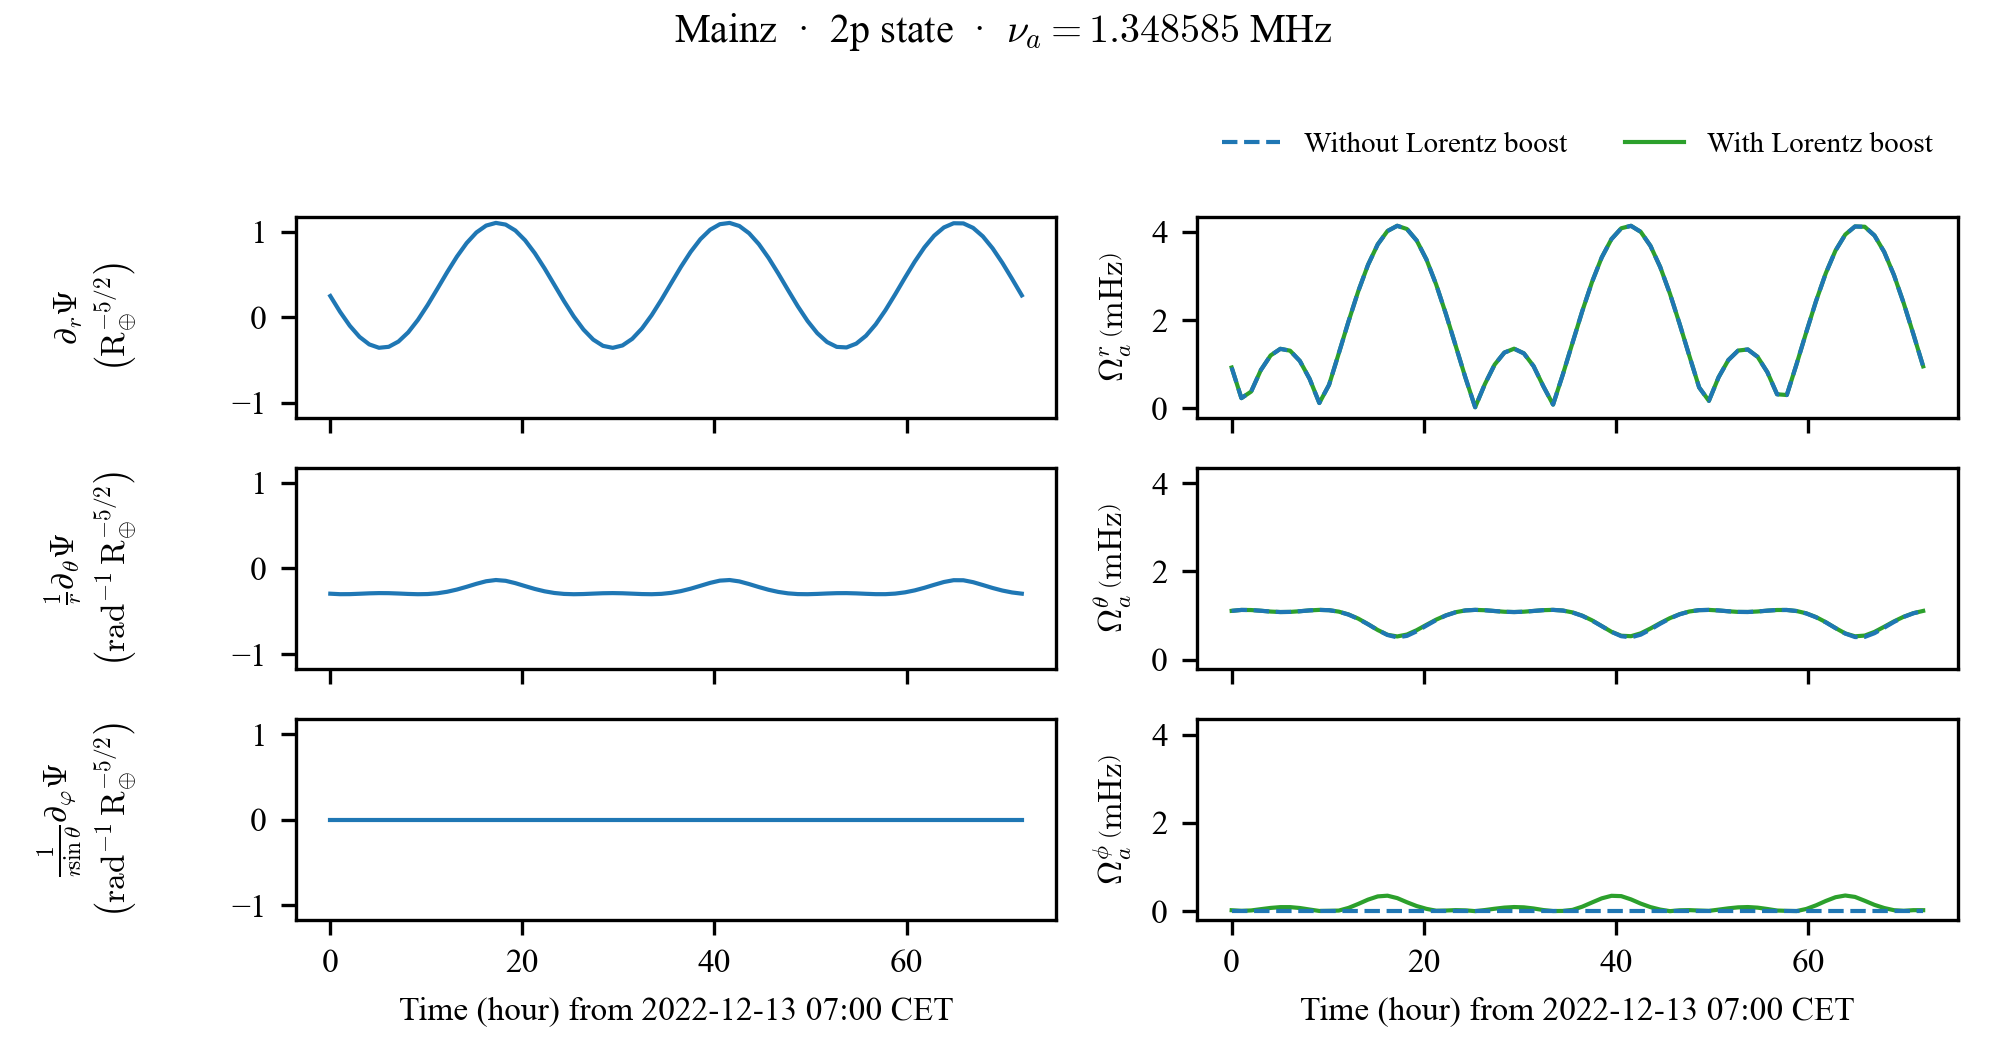
\includegraphics[width=0.99\textwidth]{figures/gradients_Omega_a_comparison_2p.png}
    \caption{gradients of 1s 2p... states.
    Three rows would be enogh.}
    \label{fig:gradients}
\end{figure}

\YZ{Add a numerical estimate for $\Omega_a^\mathrm{Earth}$ as a function of $m_a$ and $M_\mathrm{bound}$.
Add a comparison with the galactic-halo Rabi frequency $\Omega_a$ (Equation~\eqref{eq:Omega_a}).}
% estimation of the Rabi frequency $\Omega_a^\mathrm{Earth}$ for the Earth-bound ALP
A rough estimation of the Rabi frequency $\Omega_a^{\oplus}$ of the pseudomagnetic field can be made using Equation~\eqref{eq:Omega_a} and escape speed $v_\mathrm{esc}$ as the typical velocity of the Earth-bound ALP:
\begin{equation}
    \Omega_a^{\oplus} / (2 \pi)\approx \frac{g_\mathrm{aNN}}{\SI{1e-9}{\GeV^{-1}}} \times \SI{6}{\mHz}~.
    \label{eq:Omega_a_earth_rough}
\end{equation}
A more accurate estimation can be made using the numerical values of the wavefunction gradients at the detector location.
With Equations~(\ref{eq:Bpseudo}, \ref{eq:gradient_Psi_sum}, \ref{eq:gradient_psi_nlm}), it can be estimated as
\begin{equation}
    \Omega_a^{\oplus} = c\, g_\mathrm{aNN} \sqrt{\frac{N_a \hbar^3 c}{2 m_a}}\,\left|\left(\boldsymbol{\nabla}\psi_{nlm}\right)_\perp\right|
    \,,\label{eq:Omega_a_earth}
\end{equation}
where $\left|(\boldsymbol{\nabla}\psi_{nlm})_\perp\right|$ is the magnitude of the wavefunction gradient component perpendicular to the bias field $\mathbf{B}_0$ (i.e., the $\hat{\boldsymbol{\theta}}$ and $\hat{\boldsymbol{\varphi}}$ terms from Equation~\eqref{eq:gradient_psi_nlm}).
Using the numerical values of the wavefunction gradients, the value can be obtained as
\begin{equation}
    \Omega_a^{\oplus, \theta} / (2 \pi)\approx \frac{g_\mathrm{aNN}}{\SI{1e-9}{\GeV^{-1}}} \times \SI{3}{\mHz}~.
    \label{eq:Omega_a_earth_theta}
\end{equation}
\YZ{What about the radial gradient?
TODO: add it.}
The two estimations in Equation~\eqref{eq:Omega_a_earth_rough} and \eqref{eq:Omega_a_earth_theta} yield consistent results within an order of magnitude.
The calculations can be found at \YZ{add reference to the script used for the calculation}.
% scripts-and-data\grav_potential.ipynb #### Estimation of the ALP field gradient Note that due to the magnitude of the Rabi frequency can vary by \SI{100}{\percent} due to the time-changing alignment between the ALP gradient and the sensitive axis of detector.

Such Rabi frequency is $\sim$7 orders of magnitude larger than the expected Rabi frequency from the galactic halo ALP, which is $\Omega_a/(2\pi)=\frac{g_\mathrm{aNN}}{\SI{1e-9}{\GeV^{-1}}}\times\SI{2e-10}{\Hz}$, as estimated after Equation~\eqref{eq:Omega_a}\YZ{TODO: I may have to choose a different equation after finishing theory section}.
% TODO: mention local dm density and low axion speed
If indeed such amount of axionlike dark matter can be accumulated in the Earth gravitational potential, it would produce a much stronger signal than the galactic halo ALP, making it an target that CASPEr-G is sensitive to.

\subsection{Population and coherence}\label{sec:theory:earthALP:coherence}

Unlike the galactic halo signal, which has a continuous Maxwell-Boltzmann spectrum, Earth-bound ALPs occupy discrete energy levels. 
Only the lowest few eigen-states are of interest because the higher eigen-states have small wavefunction amplitudes at the detector location.
The population of the eigen-states is determined by the dark matter capture / accumulation process and potential ALP self-interaction or interactions with other particles, which is not well understood. 
The population distribution is therefore treated as a free parameter in this thesis. 
A few simple scenarios are considered: (1) only one of the lowest eigenstates are populated; (2) the first few eigenstates are populated uniformly.


Each level $n$ contributes an ALP oscillation at a slightly different Compton frequency
\begin{equation}
    \nu_n = \nu_a + \frac{|E_n|}{h}
    % = \nu_a\left(1 + \frac{\alpha_g^2}{2n^2}\right)
    \,,\label{eq:nu_bound}
\end{equation}
where $\nu_a = m_a c^2/h$ is the rest-mass Compton frequency.
% The level spacing between adjacent states $n$ and $n+1$ is
% \begin{equation}
%     \Delta\nu_n = \frac{m_a c^2\,\alpha_g^2}{h}\left(\frac{1}{2n^2} - \frac{1}{2(n+1)^2}\right)
%     \approx \frac{m_a c^2\,\alpha_g^2}{h\,n^3}
%     \,.\label{eq:level_spacing}
% \end{equation}
% \YZ{Add numerical value of $\Delta\nu_n$ for $n=1$ and the masses of interest.}

If multiple modes are populated simultaneously, the phases of the individual oscillations drift relative to each other over time. 
% their superposition produces a beating pattern with a period $\tau_\mathrm{beat} \approx 1/\Delta\nu_n$.
This leads to finite coherence time for the multi-mode ALP field. 
% : the signal amplitude fluctuates on the time scale $\tau_\mathrm{beat}$, analogous to the galactic-halo coherence time $\tau_a = Q_a/\nu_a$ but with a discrete rather than continuous spectrum. 
A rough estimate of the coherence time can be made from the spacing $\Delta E$ between eigen-states:
\begin{equation}
    \tau_\mathrm{coh} \approx \frac{1}{\Delta \nu} = \frac{h}{\Delta E}
    \,.\label{eq:coherence_time_estimate}
\end{equation}
The maximum spacing can be estimated from the ALP mass and the Earth gravitational potential which is $|\Delta V_g| = \SI{125}{\mega\joule\per\kg}$:
\begin{align}
    \Delta E &\approx m_a\,\Delta V_g \approx m_a\,\frac{G M_\oplus}{R_\oplus}\\
    & = \SI{6e-18}{\eV}\frac{\nu_a}{\SI{1}{\mega\hertz}}
    \,.\label{eq:coherence_time_estimate_max}
\end{align}
\YZ{check the value of Vg later.}
The corresponding frequency spacing and coherence time are
\begin{equation}
    \Delta\nu = \frac{\Delta E_\mathrm{max}}{h} \approx \SI{1e-9}{}\nu_a
    \,\label{eq:coherence_time_estimate_max_freq}
\end{equation}
and
\begin{equation}
    \tau_\mathrm{coh} \approx \frac{1}{\Delta\nu} = \frac{10^9}{\nu_a}
    \,.\label{eq:coherence_time_estimate_max_value}
\end{equation}
\footnote{Calculations can be found at \url{scripts-and-data/Theory-EarthHaloALP.ipynb}.}
It can be seen that the coherence time is $\sim 10^3$ times longer than the galactic-halo coherence time $\tau_a = Q_a/\nu_a \sim 10^6/\nu_a$ due to the much smaller velocity spread of the Earth-bound ALP. 

To determine the exact coherence time, numerical solutions of Equation~\eqref{eq:schrodinger_earth} and simulations of eigen-states interference are needed. 
However, when the ALP mass is small, the level spacing is small and the coherence time can be very long, which may exceed the relaxation times of the NMR sample and duration of a typical CASPEr-G measurement. 
In such scnarios, the ALP field will result in a one-bin signal in the frequency spectrum, and the amplitude of the signal will be limited by the relaxation times of the NMR sample. 
Therefore, the exact value of the coherence time is not always needed for the analysis of the CASPEr-G data. 


\subsection{Periodic modulations}\label{sec:theory:earthALP:periodic}

% assuming the ALP halo is stationary while Earth is rotating at period of a day, daily modulation of the ALP signal amplitude is expected.
% However, the numerical

The Earth-bound ALP wavefunction $\psi_{nlm}$ is defined in the Earth-centered frame introduced above, with the $z$-axis along the Earth--Sun line, the $x$-axis along the instantaneous velocity of the Earth in the Solar System, and $\hat{\mathbf{y}}=\hat{\mathbf{z}}\times\hat{\mathbf{x}}$.
This frame is generally not aligned with the Earth's rotation axis.
As the Earth rotates, the laboratory co-rotates, so the orientation of the component of $\boldsymbol{\nabla}a$ at any given location therefore exhibits a daily modulation. 
% For a bias field pointed along the local vertical, and a bound state with quantum numbers $(n, l, m)$, the perpendicular gradient component traces a specific daily pattern determined by the spherical harmonic $Y_l^m$ evaluated at the detector's co-latitude \YZ{add explicit formula for the modulation amplitude as a function of co-latitude and $(l,m)$}.
% This daily modulation is a powerful discriminant: its period (one sidereal day) and phase are fixed by Earth's rotation and the quantum numbers of the bound state, providing a strong consistency check that is qualitatively different from both the galactic-halo signal (which has a different daily modulation driven by the velocity of the halo wind, cf.\ Section~\ref{sec:theory:earthALP:periodic}) and instrumental artifacts.
\YZ{Add figure: predicted daily modulation envelope for the ground state at a mid-latitude detector, for one or two representative masses.}

One example of daily modulation is illustrated in Figure~\ref{fig:earthALP_daily_modulation}, which shows the daily modulation of gradient component for the $2p$ state $(n, l, m) = (2, 1, 0)$ at the location of CASPEr-G. 

\begin{figure}
    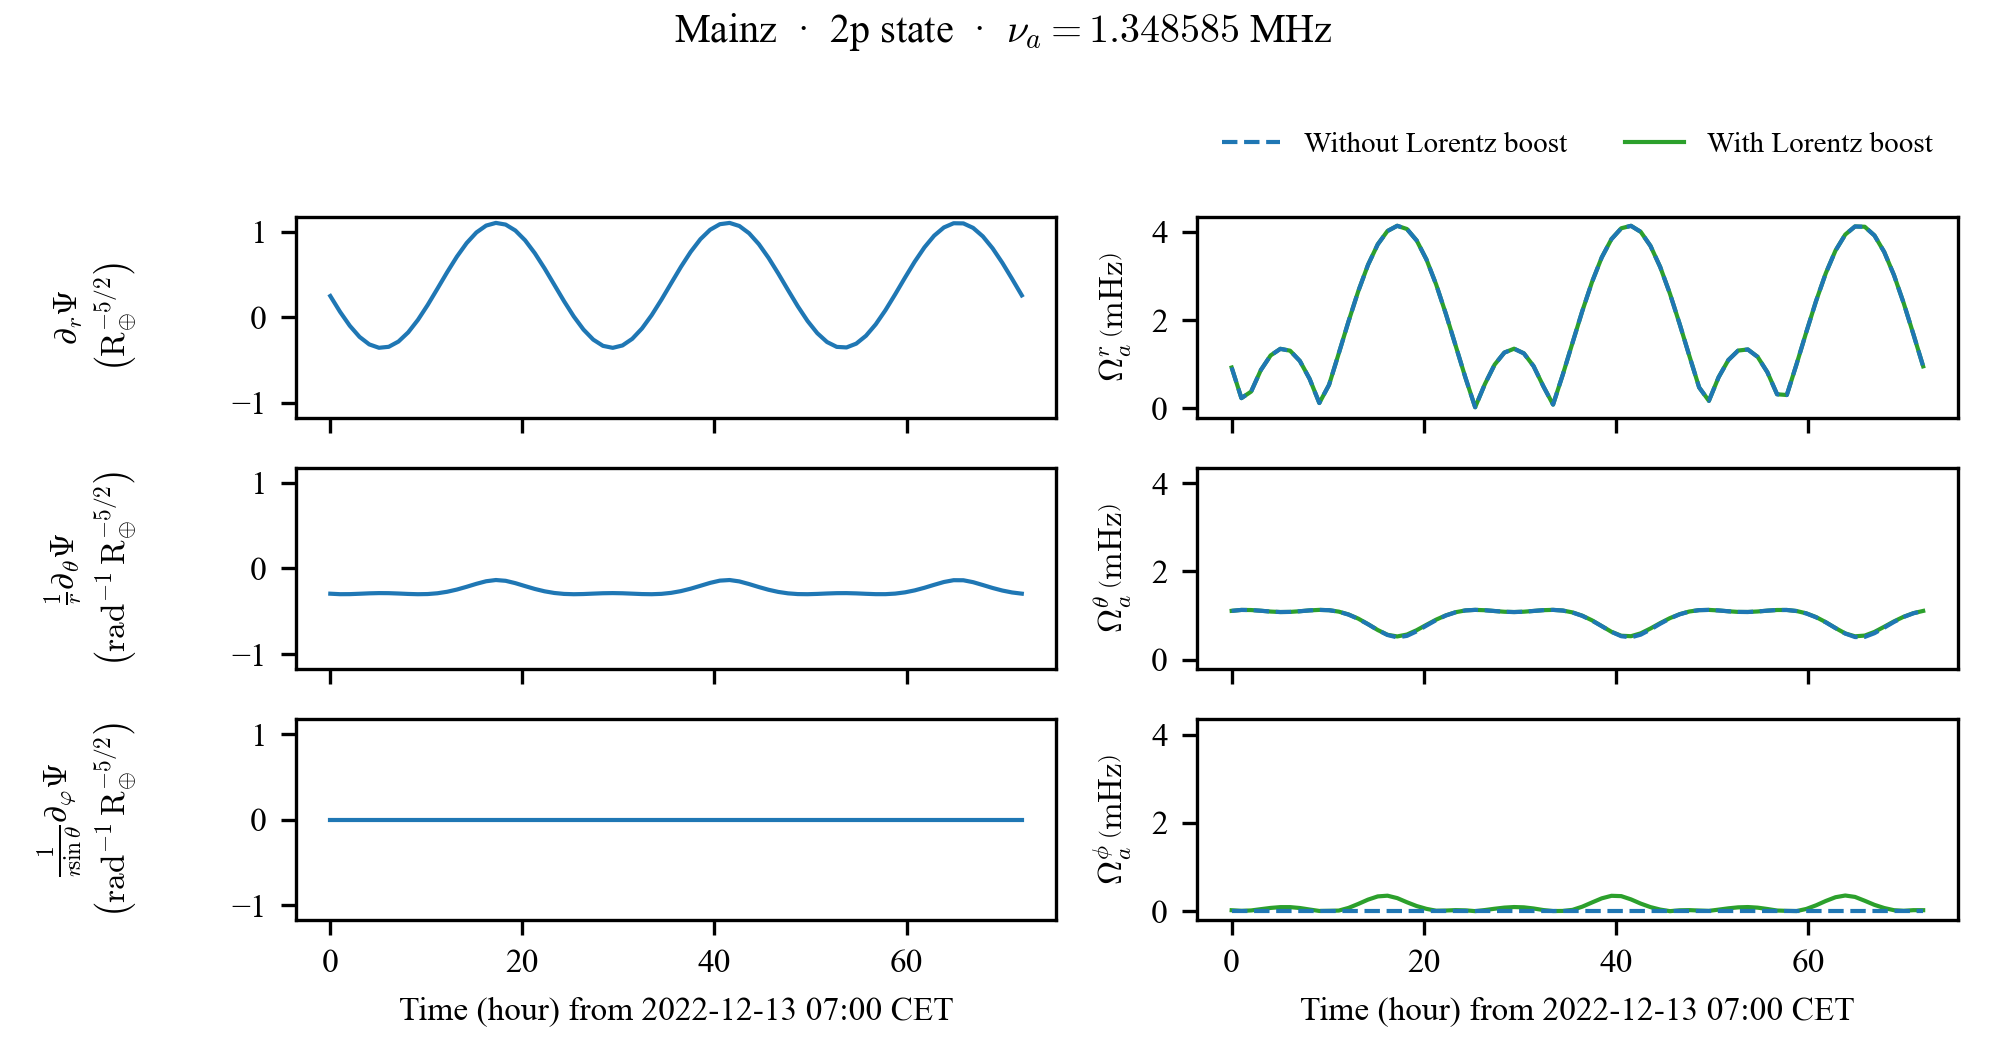
\includegraphics[width=0.99\textwidth]{figures/gradients_Omega_a_comparison_2p.png}
    \caption{Daily modulation of the gradient component for the $2p$ state $(n, l, m) = (2, 1, 0)$ at the location of CASPEr-G (Helmholtz Institute Mainz). 
    The modulation is due to the rotation of the Earth.}
    \label{fig:earthALP_daily_modulation}
\end{figure}
